\chapter{Pustaka \texttt{Scikit-Image}}
\section{Pendahuluan}

Saat diktat ini disusun, versi stabil terbaru dari pustaka \texttt{scikit-image} adalah \texttt{0.16.2}. Diktat ini disusunan berdasarkan penjelasan yang disajikan di \url{https://scikit-image.org/}. Sedangkan alur penyajiannya didasarkan pada kebutuhan untuk mendapatkan fitur citra.

Seperti dijelaskan \cite{Gonzalez}, pengolahan citra mentargetkan kemampuan pengenalan obyek seperti dijelaskan pada \figurename~\ref{fig:targetProcessing}. Fitur yang berhasil diekstraksi dari berbagai metode pengolahan citra akan menjadi masukan bagi pustakan Python lain seperti \texttt{scikit-learn} dan \texttt{tensorflow}.

\begin{figure}[h!]
  \begin{center}
    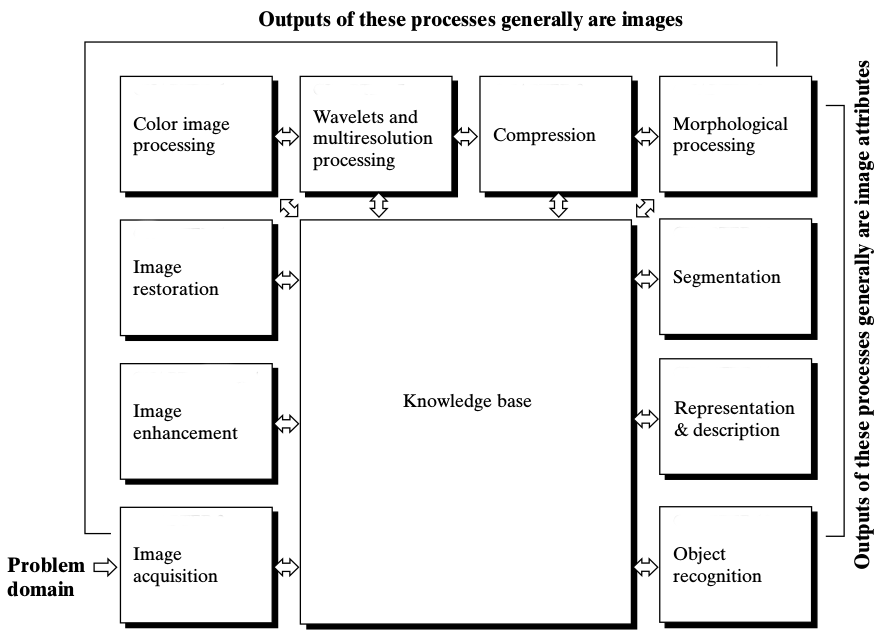
\includegraphics[scale=.5]{pics/steps.png}
    \caption{Pengeolahan citra untuk pengenalan obyek \cite{Gonzalez}}
    \label{fig:targetProcessing}
  \end{center}
\end{figure}

\section{Sub modul I/O}
Penjelasan tentang pengolahan citra berbasis \texttt{scikit-image} akan dimulai dengan sub module I/O (\textit{Input}/\textit{Output}). Pengguna harus memahami cara \texttt{scikit-image} membaca sebuah citra dan representasi dari pembacaan tersebut dalam komputer.
